\addcontentsline{toc}{chapter}{Anhang} %sorgt für eintrag ins inhaltsverzeichnis
\chapter{Ergänzungen zur Forschungsfrage eins} \label{appendixFF1}
In diesem Teil des Anhangs sind Ergänzungen zur Forschungsfrage zwei des Kapitels \vref{ff2} beschrieben.

\section{Anforderungsdokument}\label{appendixAnforderung}

Ein Anforderungskatalog hat bestimmte Anforderungen, die an den Katalog gestellt werden. Neben der Forderung nach Einhaltung der Qualitätskriterien, definiert nach dem ISO-Standard 9000/9001, sind noch folgende Forderungen in der Literatur beschrieben: \autocite[sig.][S.34]{partsch_requirements-engineering_2010}

\begin{itemize}
	\item vollständig (inhaltlich – d. h., alle Anforderungen sind erfasst –, formal, Norm-konform)
	\item konsistent (keine Widersprüche zwischen den Bestandteilen des Dokuments,
	insbesondere keine Konflikte zwischen verschiedenen Anforderungen)
	\item lokal änderbar (Änderungen an einer Stelle sollten keine Einflüsse auf Konsistenz und Vollständigkeit des Gesamtdokuments haben)
	\item verfolgbar (ursprüngliche Stakeholderwünsche und Zusammenhänge zwischen
	Anforderungen sind leicht zu finden)
	\item klar strukturiert
	\item umfangsmäßig angemessen
	\item sortierbar/projezierbar (nach verschiedenen Kriterien, für verschiedene Stakeholder).
\end{itemize}

Die folgende Aufzählung beschreibt eine Vorlage für das Anforderungsdokument nach Quelle: Sie nutzt die Hilfsmittelsammlung \enquote{Volere}. Diese bietet im Themenbereich \enquote{requirements engineering} kostenpflichtig Dokumentenvorlagen an. Die beiden Bekanntesten sind die hier gezeigte \enquote{Volere Requirements Specification Template} und das kostenlose \enquote{Volere Atomic Requirement Template}, das umgangssprachlich \enquote{Snow Card} genannt wird. Die \enquote{Snow Card} (\vref{abb:volereSnowCard}) ist eine Karteikarte, die benutzt wird, um eine vollständige Aufnahme aller Informationen einer einzelnen Anforderung zu gewährleisten.\autocite[vgl.][]{VolereSnowCard} Die folgende Liste wurde in Anlehnung an die Quelle \cite{VolereRequirmentsSpecTemplate} erstellt.

\begin{minipage}{\linewidth}
	\begin{itemize}\label{abb:volereReqSpec}
		\item Projekt-Treiber
		\begin{enumerate}
			\item Zweck des Projekts
			\item Auftraggeber, Kunde und andere Stakeholder
			\item Nutzer des Produkts
		\end{enumerate}
		\item Projekt-Randbedingungen
		\begin{enumerate}
			\item Einschränkungen
			\item Namenskonventionen und Definitionen
			\item Relevante Fakten und Annahmen
		\end{enumerate}
		\item Funktionale Anforderungen
		\begin{enumerate}
			\item Arbeitsrahmen
			\item Systemgrenzen
			\item Funktionale und Daten-Anforderungen
		\end{enumerate}
		\item Nicht-funktionale Anforderungen
		\begin{enumerate}
			\item Look-and-Feel-Anforderungen
			\item Usability-Anforderungen
			\item Performanz-Anforderungen
			\item Operationale und Umfeld-Anforderungen
			\item Wartungs- und Unterstützungsanforderungen
			\item Sicherheitsanforderungen
			\item Kulturelle und politische Anforderungen
			\item Rechtliche Anforderungen
		\end{enumerate}
		\item Projekt-Aspekte
		\begin{enumerate}
			\item Offene Punkte
			\item Standardlösungen
			\item Neu aufgetretene Probleme
			\item Installationsaufgaben
			\item Migrationstätigkeiten
			\item Risiken
			\item Kosten
			\item Nutzerdokumentation
			\item Zurückgestellte Anforderungen
			\item Lösungsideen
		\end{enumerate}
	\end{itemize}
\end{minipage}


\begin{figure}[H]
	\centering
	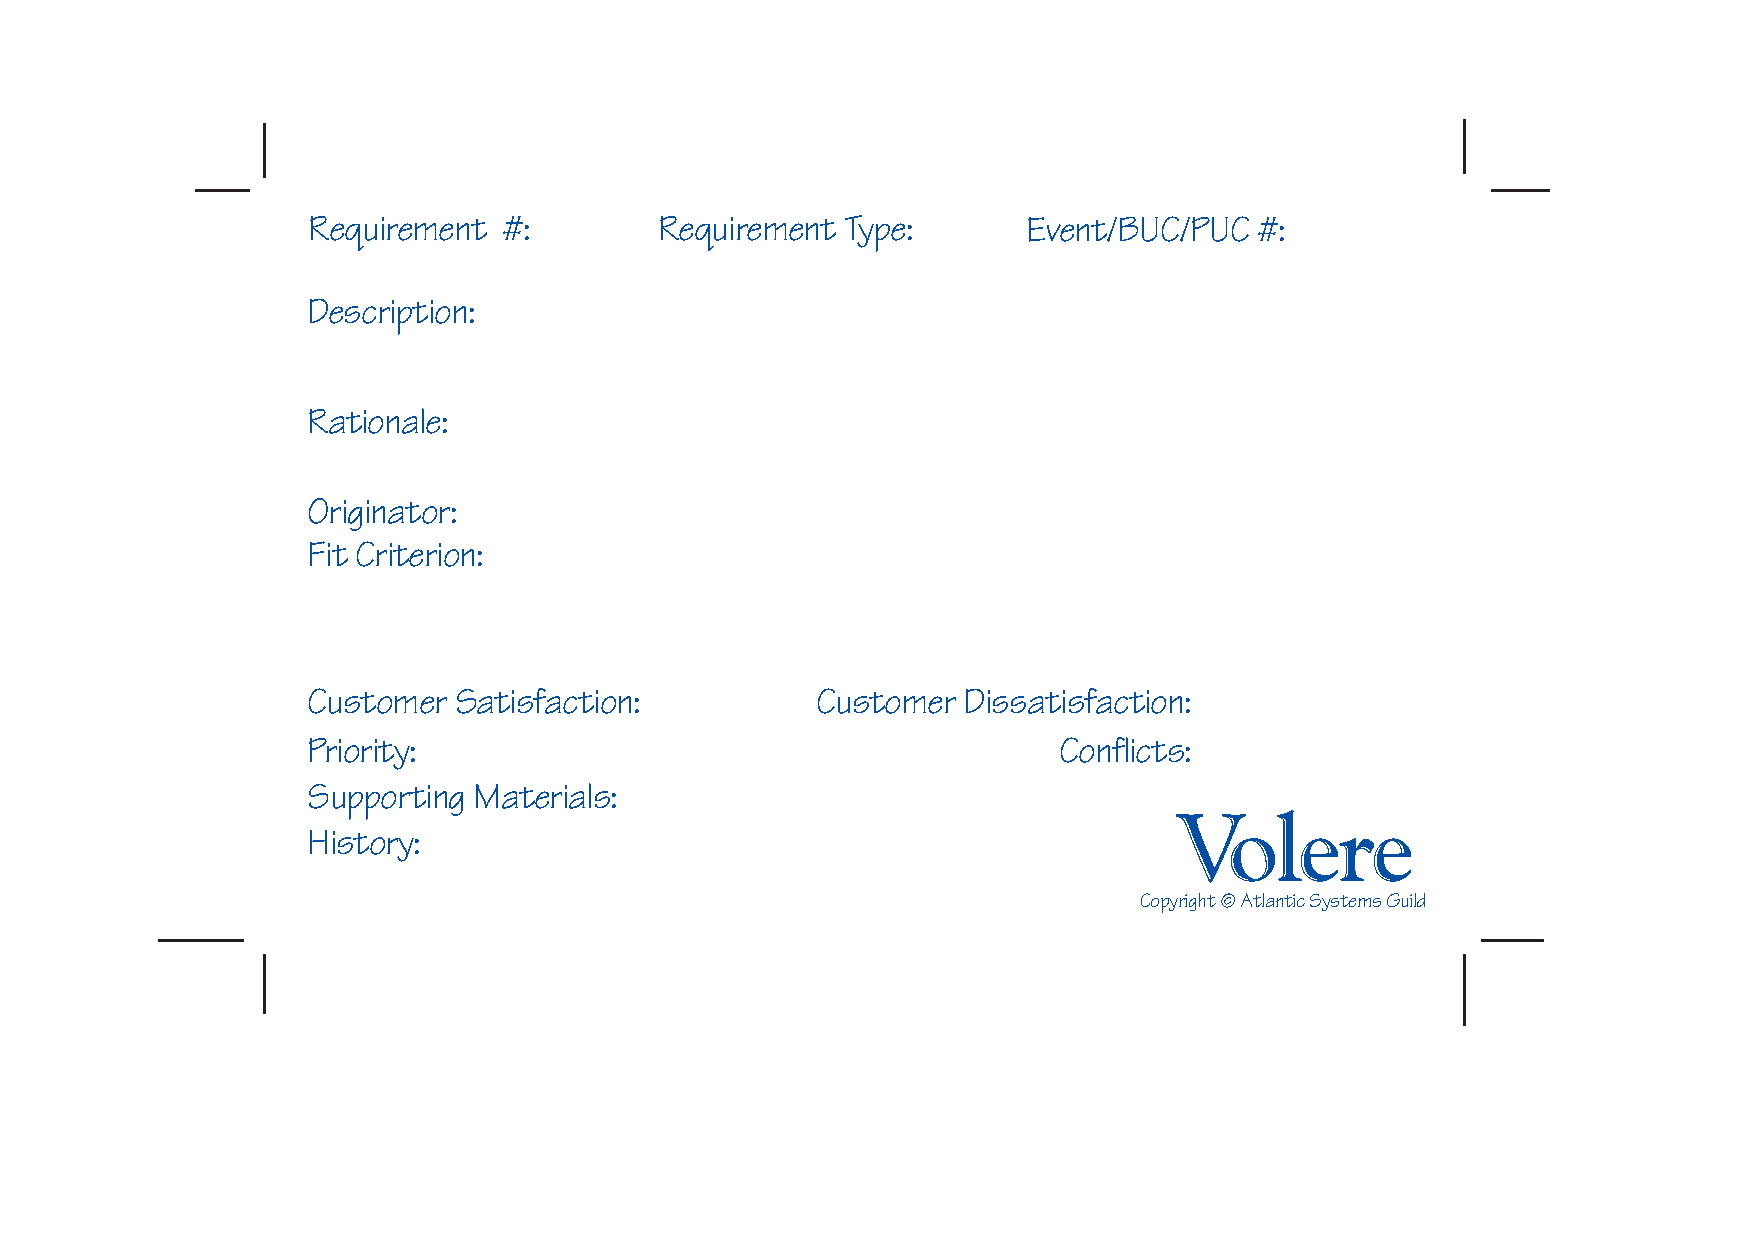
\includegraphics[scale=0.6]{img/snowcard.pdf}
	\caption{Volere Snow Card}
	{\footnotesize Quelle: \cite{VolereSnowCard}}
	\label{abb:volereSnowCard}
	%		{\scriptsize \textit{Alle Rechte, einschließlich der Vervielfältigung, Veröffentlichung, Bearbeitung und Übersetzung bleiben der SV Informatik GmbH vorbehalten.}}
\end{figure}

\begin{figure}[H]
	\centering
	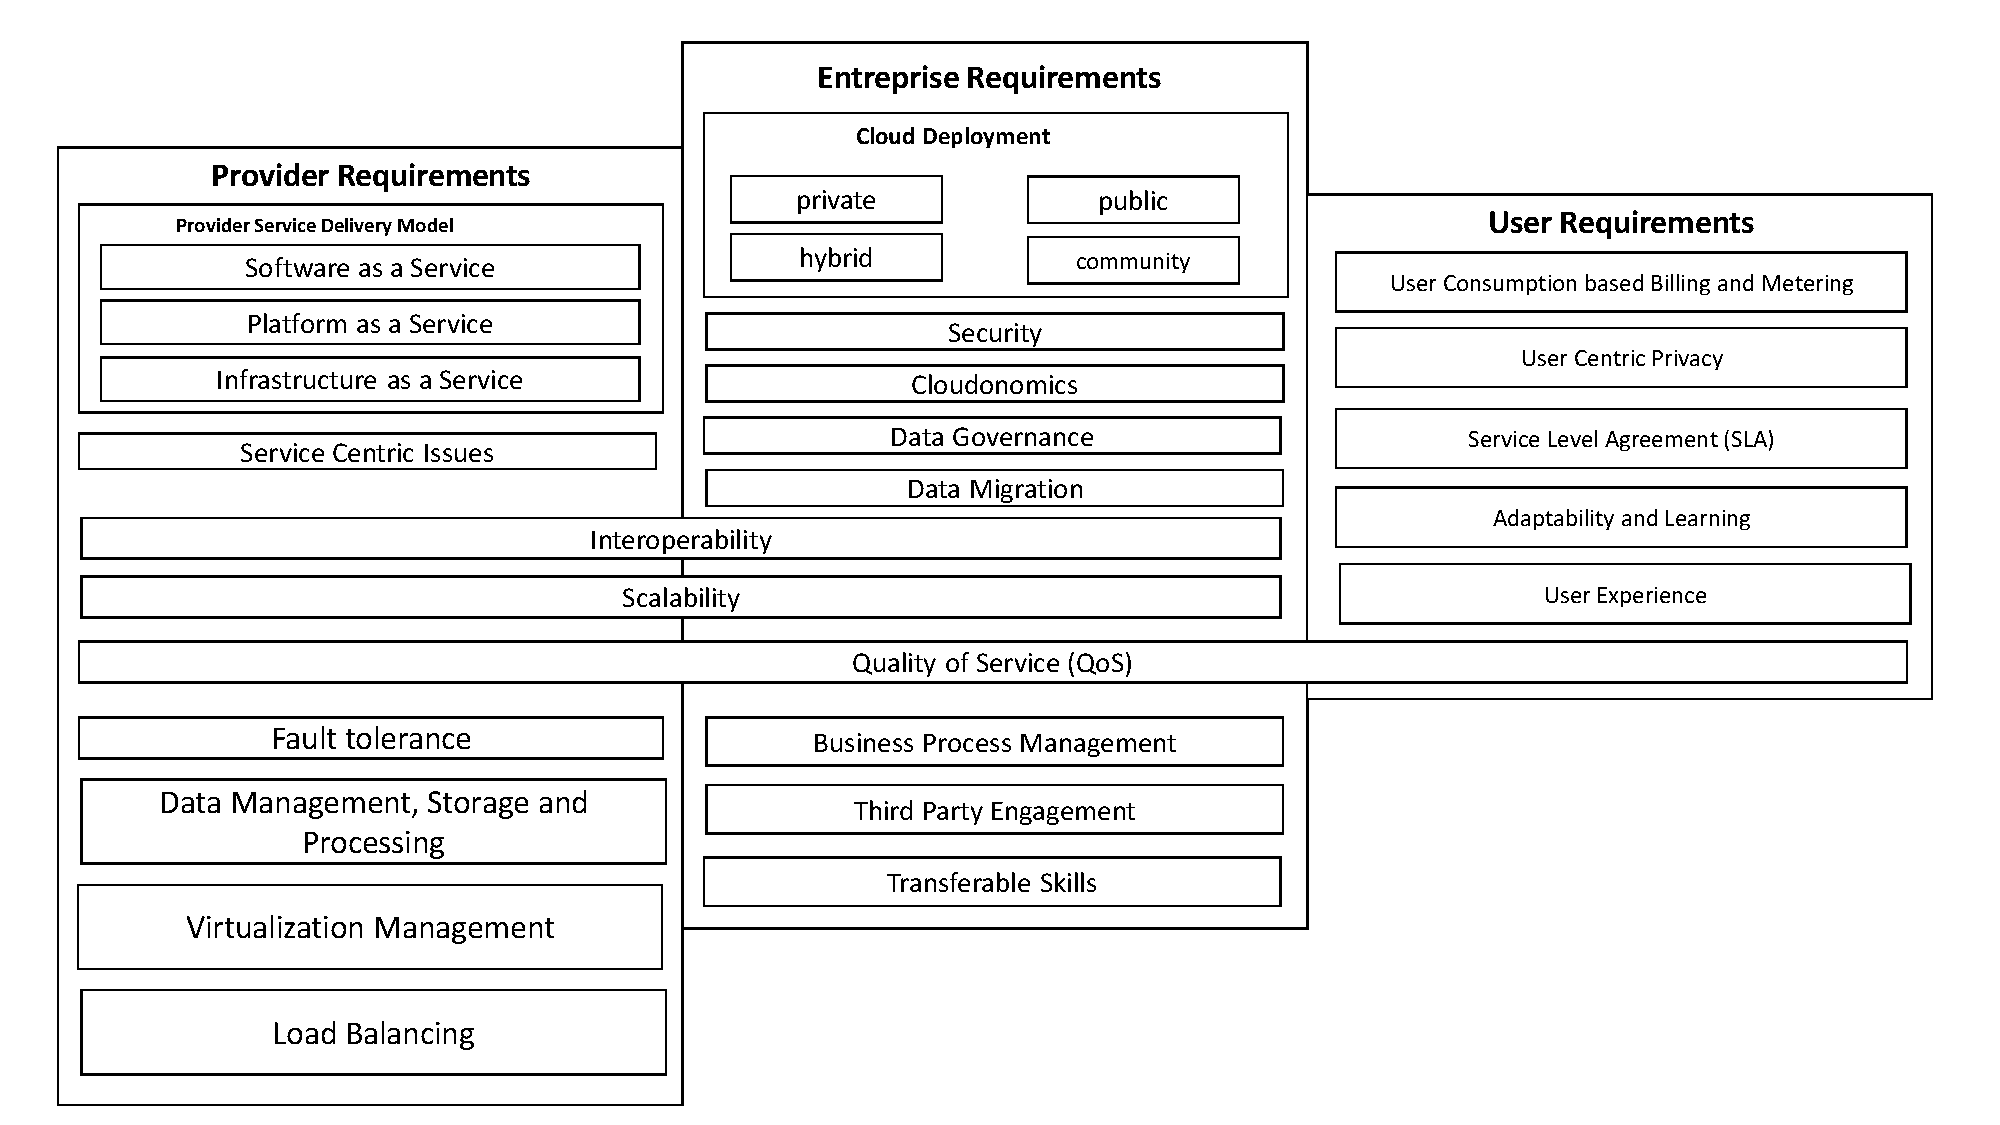
\includegraphics[scale=0.45]{img/cloudreq.pdf}
	\caption{Volere Snow Card}
	{\footnotesize Quelle: in Anlehnung an \cite{rimal_architectural_2011}}
	\label{abb:cloudreq}
	%		{\scriptsize \textit{Alle Rechte, einschließlich der Vervielfältigung, Veröffentlichung, Bearbeitung und Übersetzung bleiben der SV Informatik GmbH vorbehalten.}}
\end{figure}

\section{Statistiken zum Themengebiet \ac{Cloud-C}}

\begin{figure}[H]
	\centering
	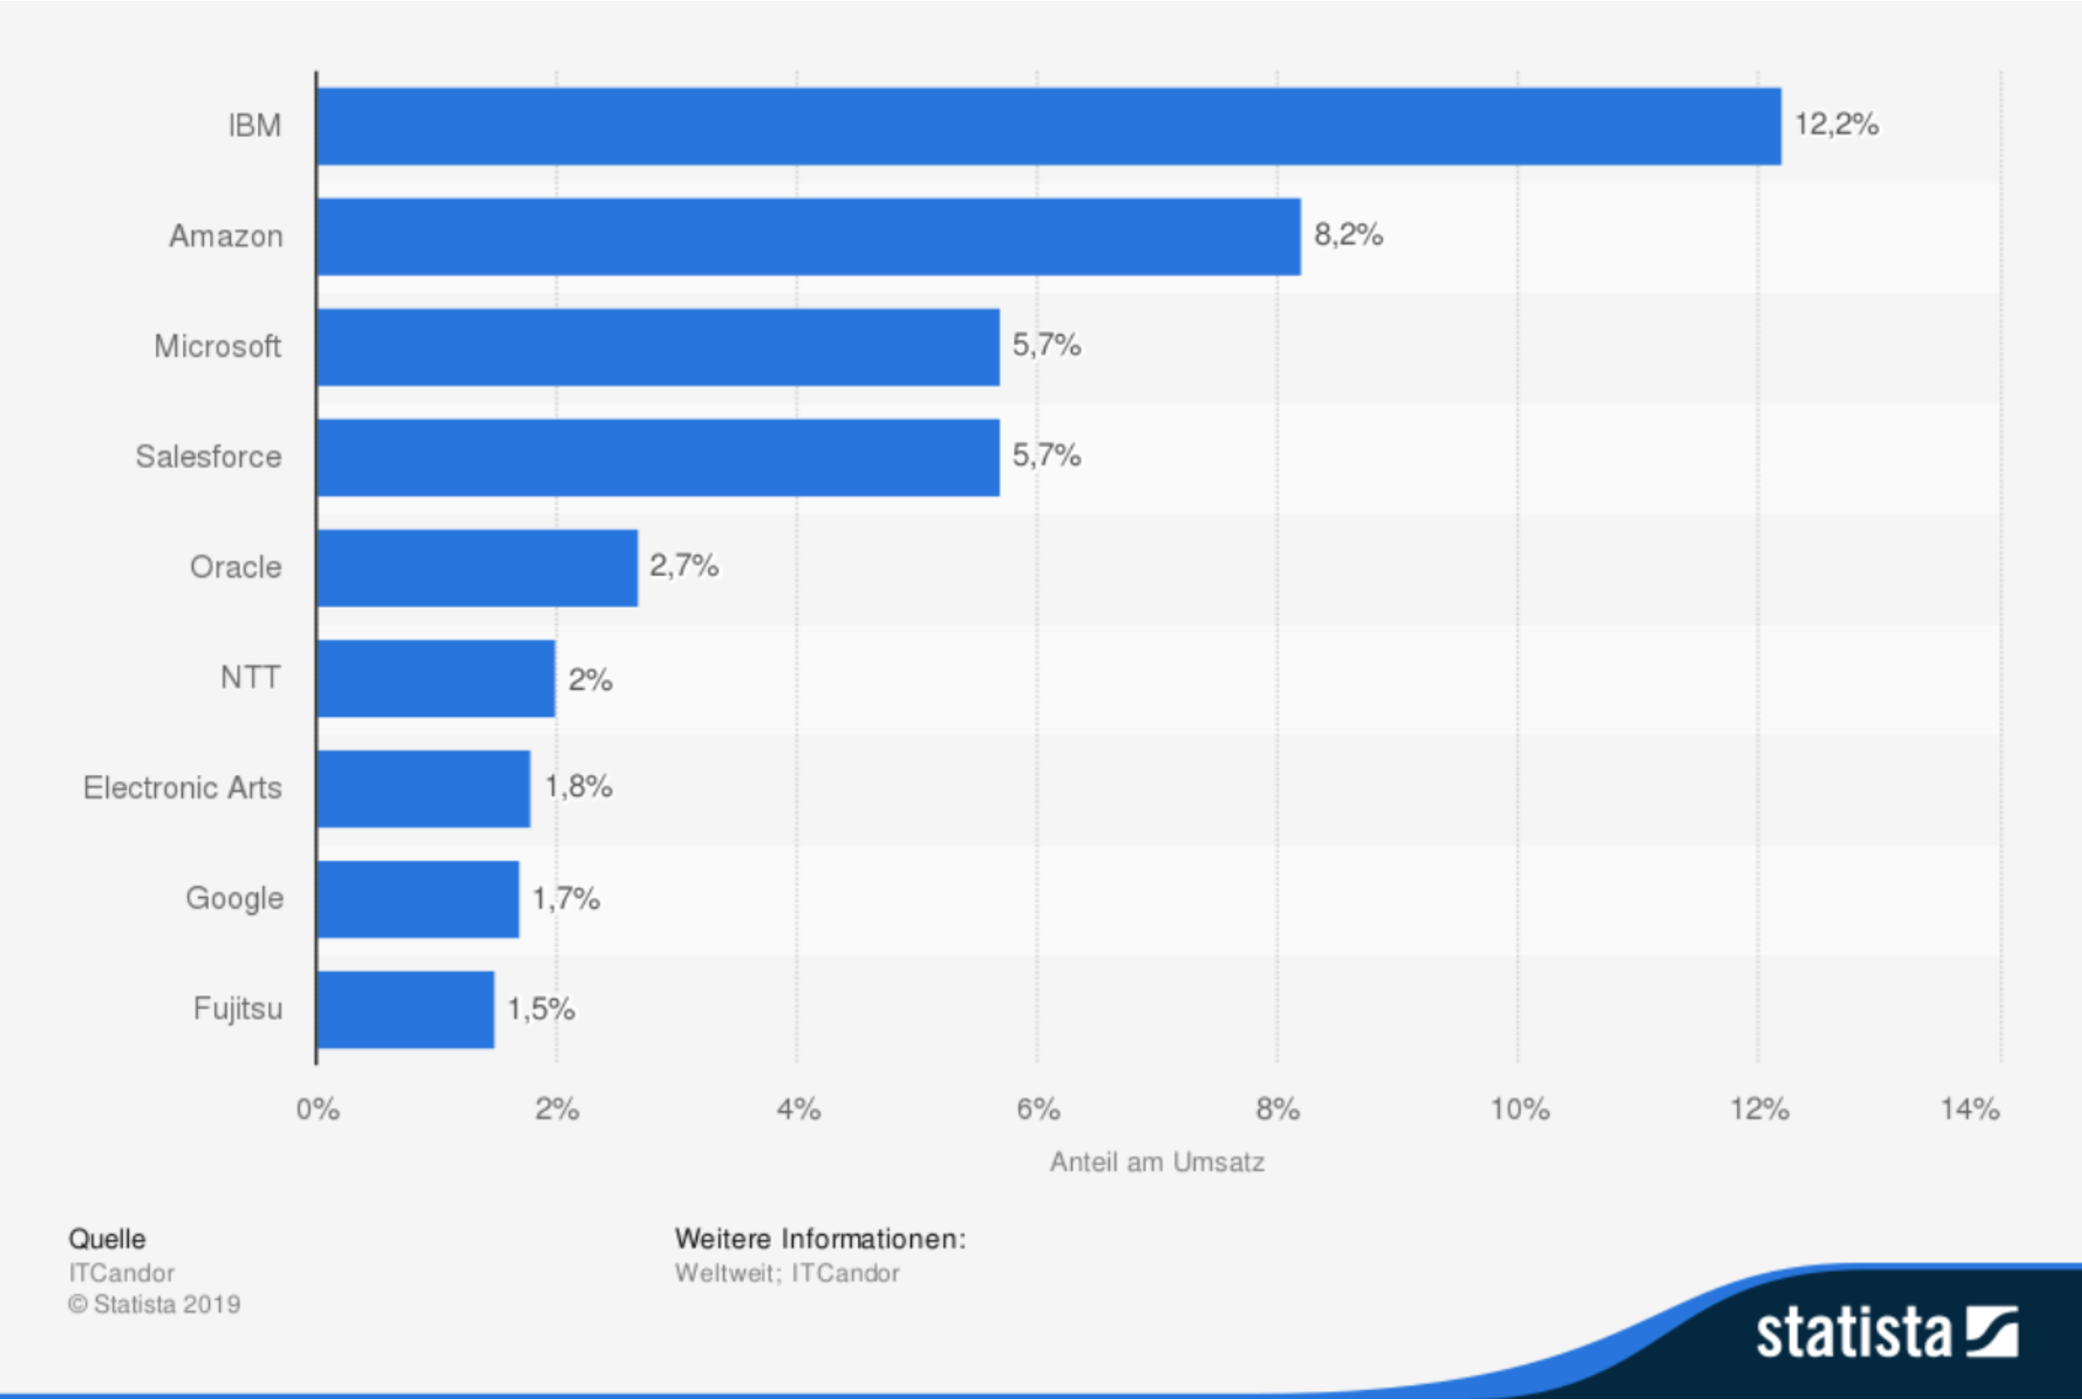
\includegraphics[scale=0.43]{img/statistic_id150979_marktanteile-der-fuehrenden-unternehmen-im-bereich-cloud-computing-weltweit-2019.pdf}
	\caption{Marktanteile der führenden Unternehmen am Umsatz im Bereich Cloud Computing weltweit von Juli 2018 bis Juni 2019}
	{\footnotesize Quelle: \cite{itcandor_cloud_2019}}
	\label{abb:marktanteileCC19}
	%		{\scriptsize \textit{Alle Rechte, einschließlich der Vervielfältigung, Veröffentlichung, Bearbeitung und Übersetzung bleiben der SV Informatik GmbH vorbehalten.}}
\end{figure}

\begin{figure}[H]
	\centering
	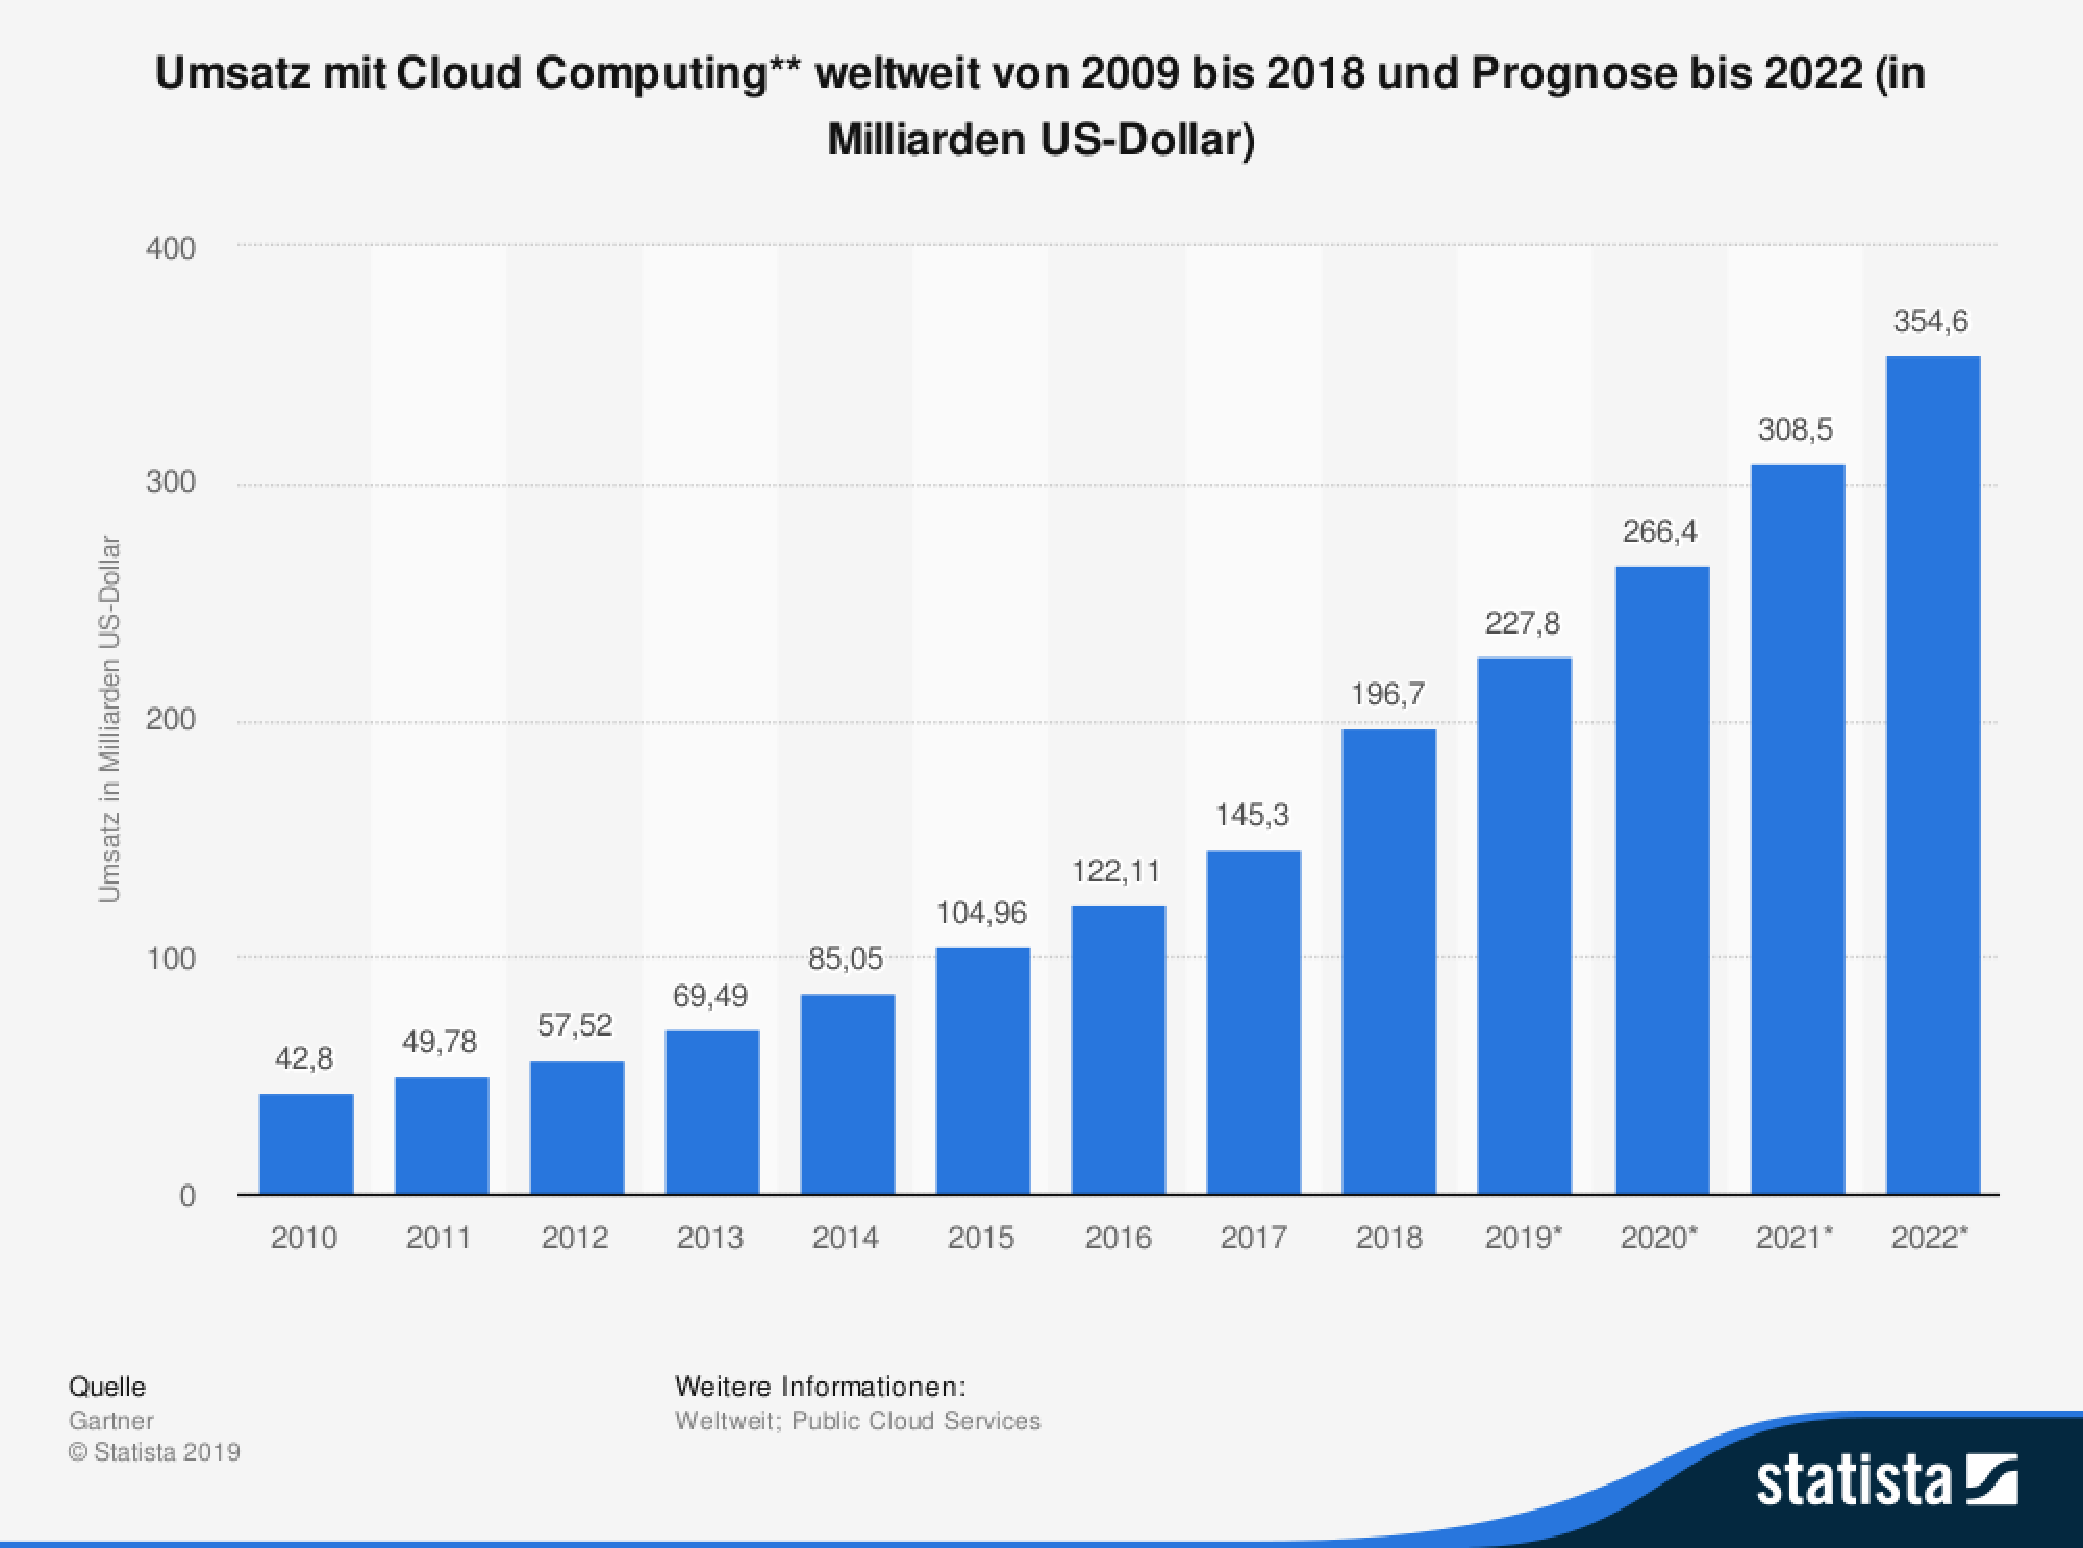
\includegraphics[scale=0.43]{img/statistic_id195760_prognose-zum-umsatz-mit-cloud-computing-weltweit-bis-2022.pdf}
	\caption{Umsatz mit Cloud-Computing weltweit von 2009 bis 2018 und Prognose bis 2022 }
	{\footnotesize Quelle: \cite{gartner_cloud_2019}}
	\label{abb:umsatzprognoseCC}
	%		{\scriptsize \textit{Alle Rechte, einschließlich der Vervielfältigung, Veröffentlichung, Bearbeitung und Übersetzung bleiben der SV Informatik GmbH vorbehalten.}}
\end{figure}

\section{Ergänzungen zum Kapitel Container(-isierung) und Orchestrierung}

\begin{figure}[H]
	\centering
	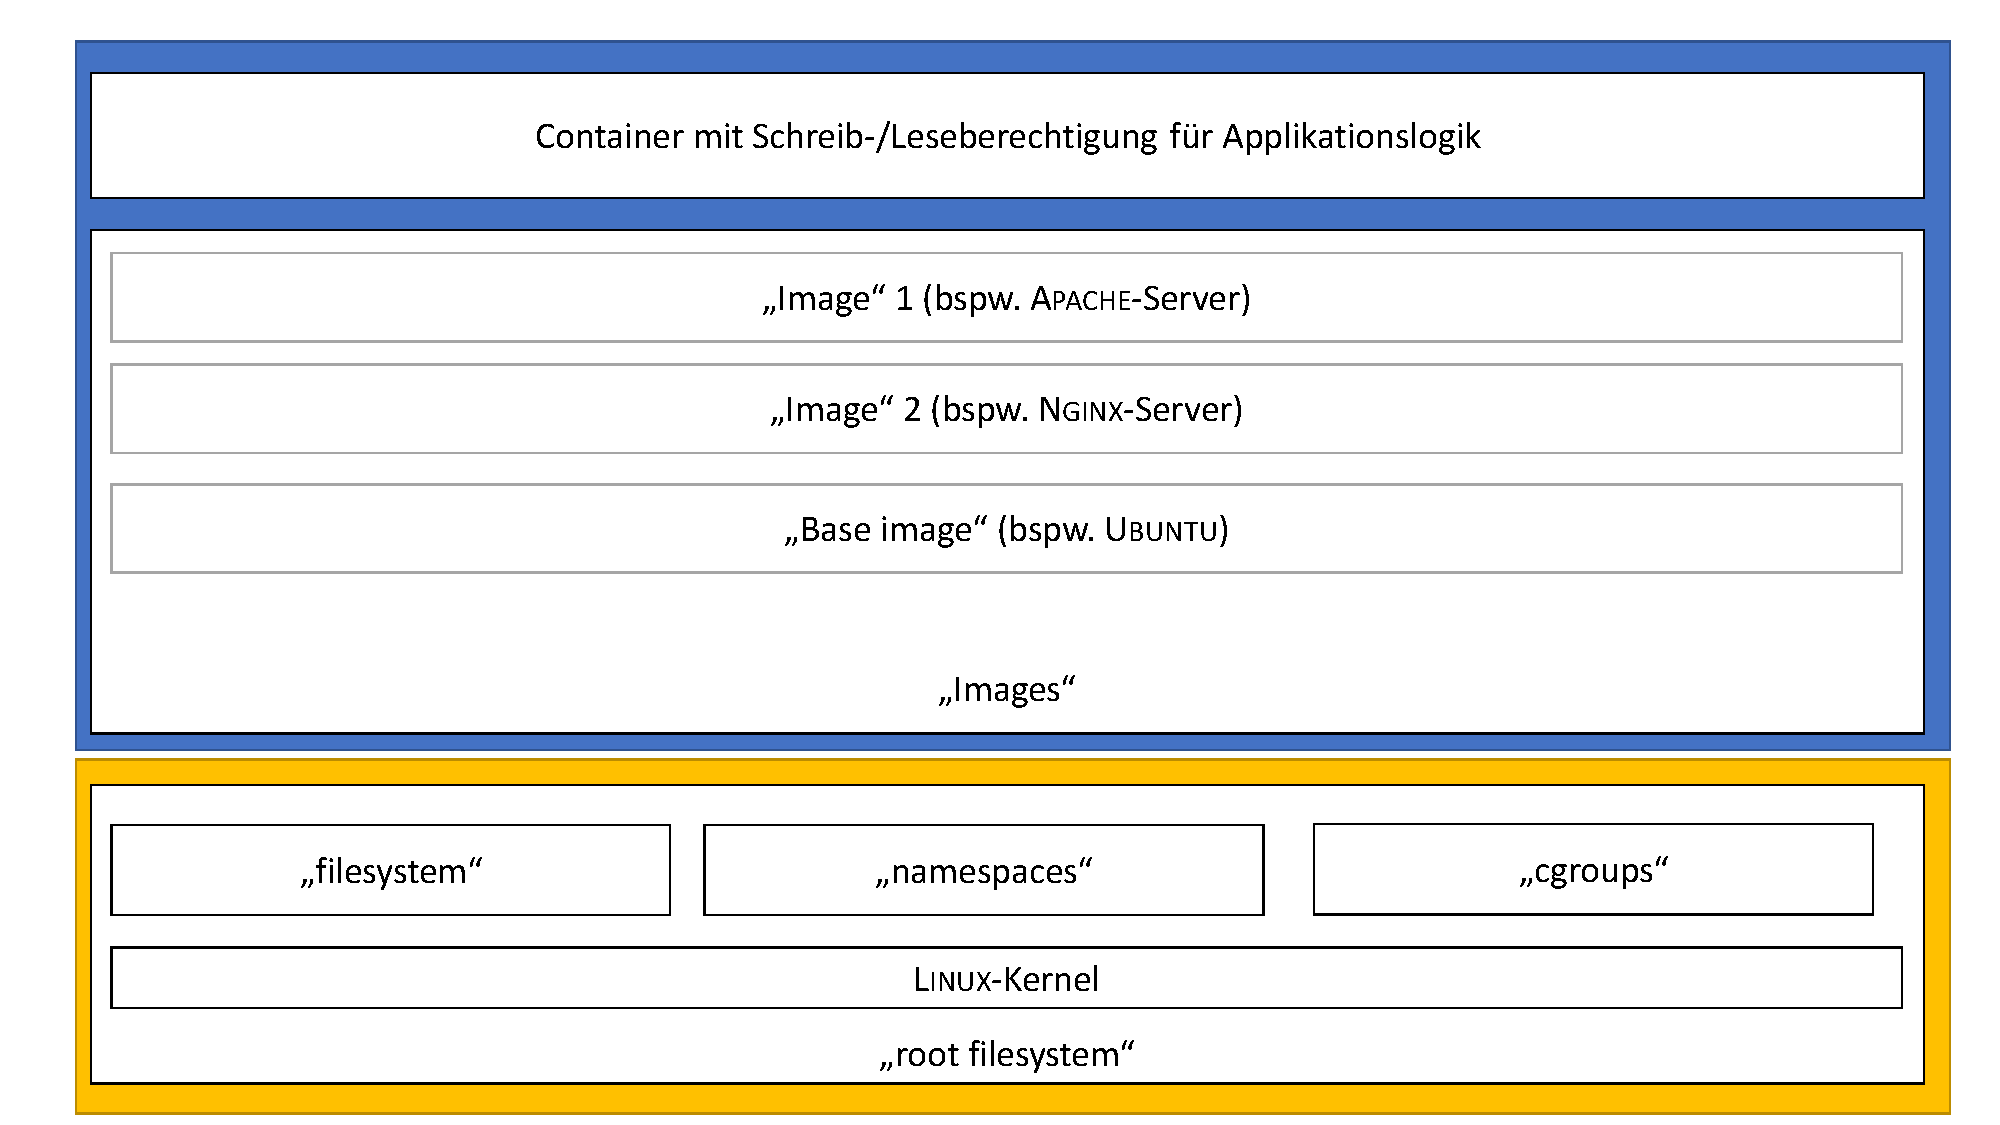
\includegraphics[scale=0.45]{img/containerImageArch.pdf}
	\caption{Architektur des Container-\enquote{Images}}
	{\footnotesize Quelle: in Anlehnung an \cite{pahl_containerization_2015}}
	\label{abb:containerArch}
	%		{\scriptsize \textit{Alle Rechte, einschließlich der Vervielfältigung, Veröffentlichung, Bearbeitung und Übersetzung bleiben der SV Informatik GmbH vorbehalten.}}
\end{figure}

Hierbei ist zu beachten, dass das orange gefärbte die Funktionalitäten der \textsc{Docker}-\enquote{Engine} und das blau gefärbte die möglichen Bestandteile eines \textsc{Docker}-\enquote{Images} darstellen soll.


\begin{figure}[H]
	\centering
	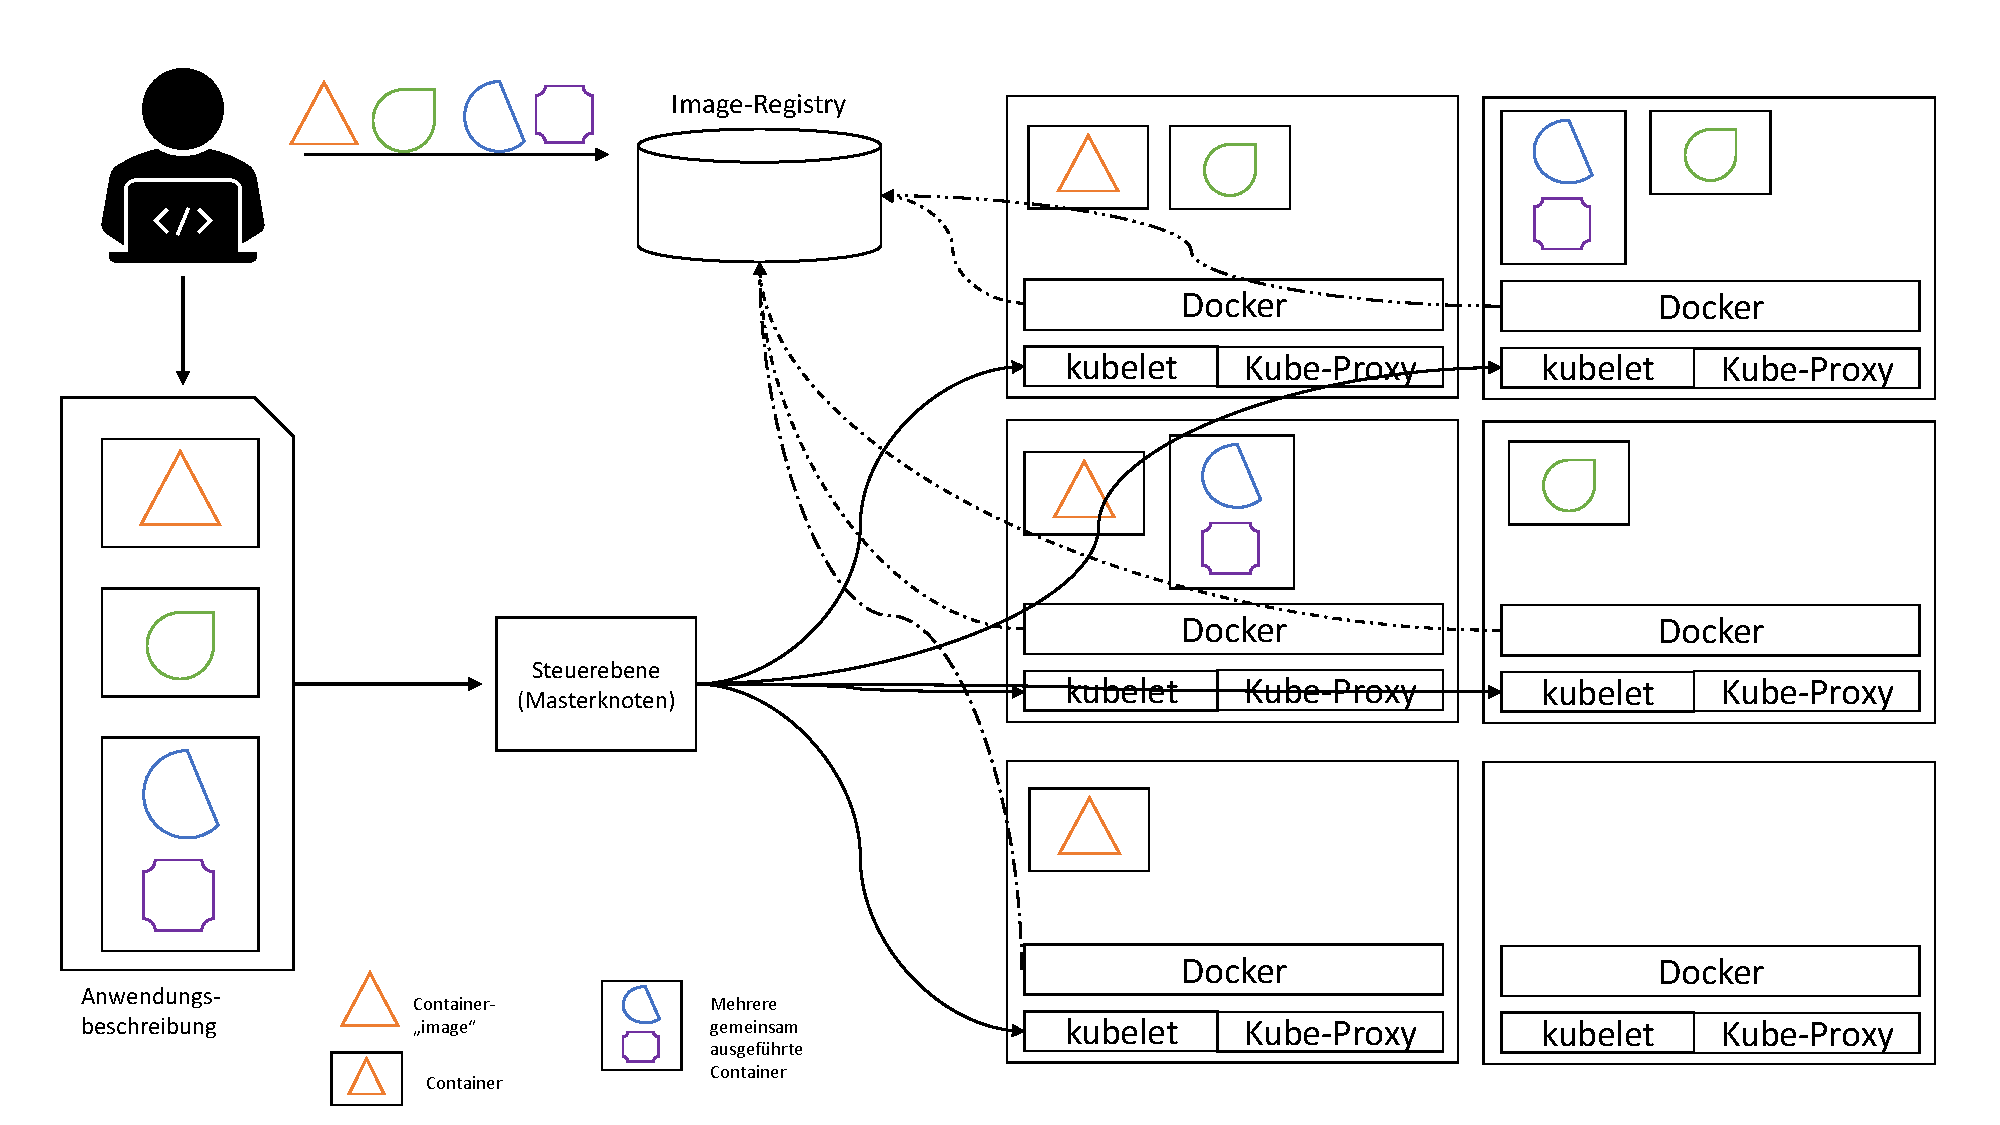
\includegraphics[scale=0.46]{img/k8sArch.pdf}
	\caption{Überblick über eine \textsc{Kubernetes}-Architektur}
	{\footnotesize Quelle: in Anlehnung an \cite[][S.23]{luksa_kubernetes_2018}}
	\label{abb:k8sArch}
	%		{\scriptsize \textit{Alle Rechte, einschließlich der Vervielfältigung, Veröffentlichung, Bearbeitung und Übersetzung bleiben der SV Informatik GmbH vorbehalten.}}
\end{figure}

\chapter{Ergänzungen zur Forschungsfrage zwei} \label{appendixFF2}



\chapter{Ergänzungen zur Forschungsfrage drei} \label{appendixFF3}


